Our program can make the robot explore most of the map, the issues still present are the fact that when we compute a path we stop the robot to avoid it going into obstacles.
That can be annoying because the robot will stop every 5 seconds since we compute the path every 5 seconds.

An other issue is the fact that we only consider the frontiers with more than 20 points in it, this becomes an issue when we want the robot to explore little areas.
The robot then performs better when it has to explore a big part of the map.

An other issue is the way that we select the frontier, indeed we select the closest frontier from the robot, sometimes the closest frontier is behind a wall.
When we are in that case an other issue appears, the fact that the A* algorithm will sometimes find a path that goes through a wall (When the wall is not yet fully discovered), leading the robot to stay stuck.
A way of correcting that issue would have been to create a map on which the obstacles are expanded which would have make it easier to find a correct path.

Under we can see a map almost fully explored by the robot.

\FloatBarrier
\begin{figure}
    \centering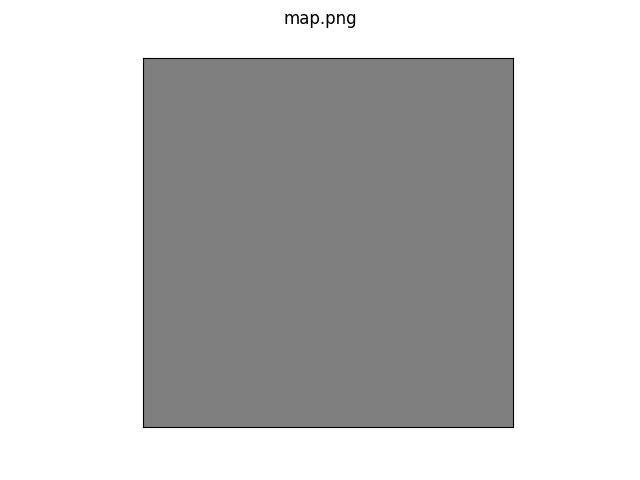
\includegraphics[width=0.5\textwidth]{map.png}
    \label{fig:map}
    \caption{Map almost fully explored}
\end{figure}
\FloatBarrier

Under we can see the robot while exploring a map.

\FloatBarrier
\begin{figure}
    \centering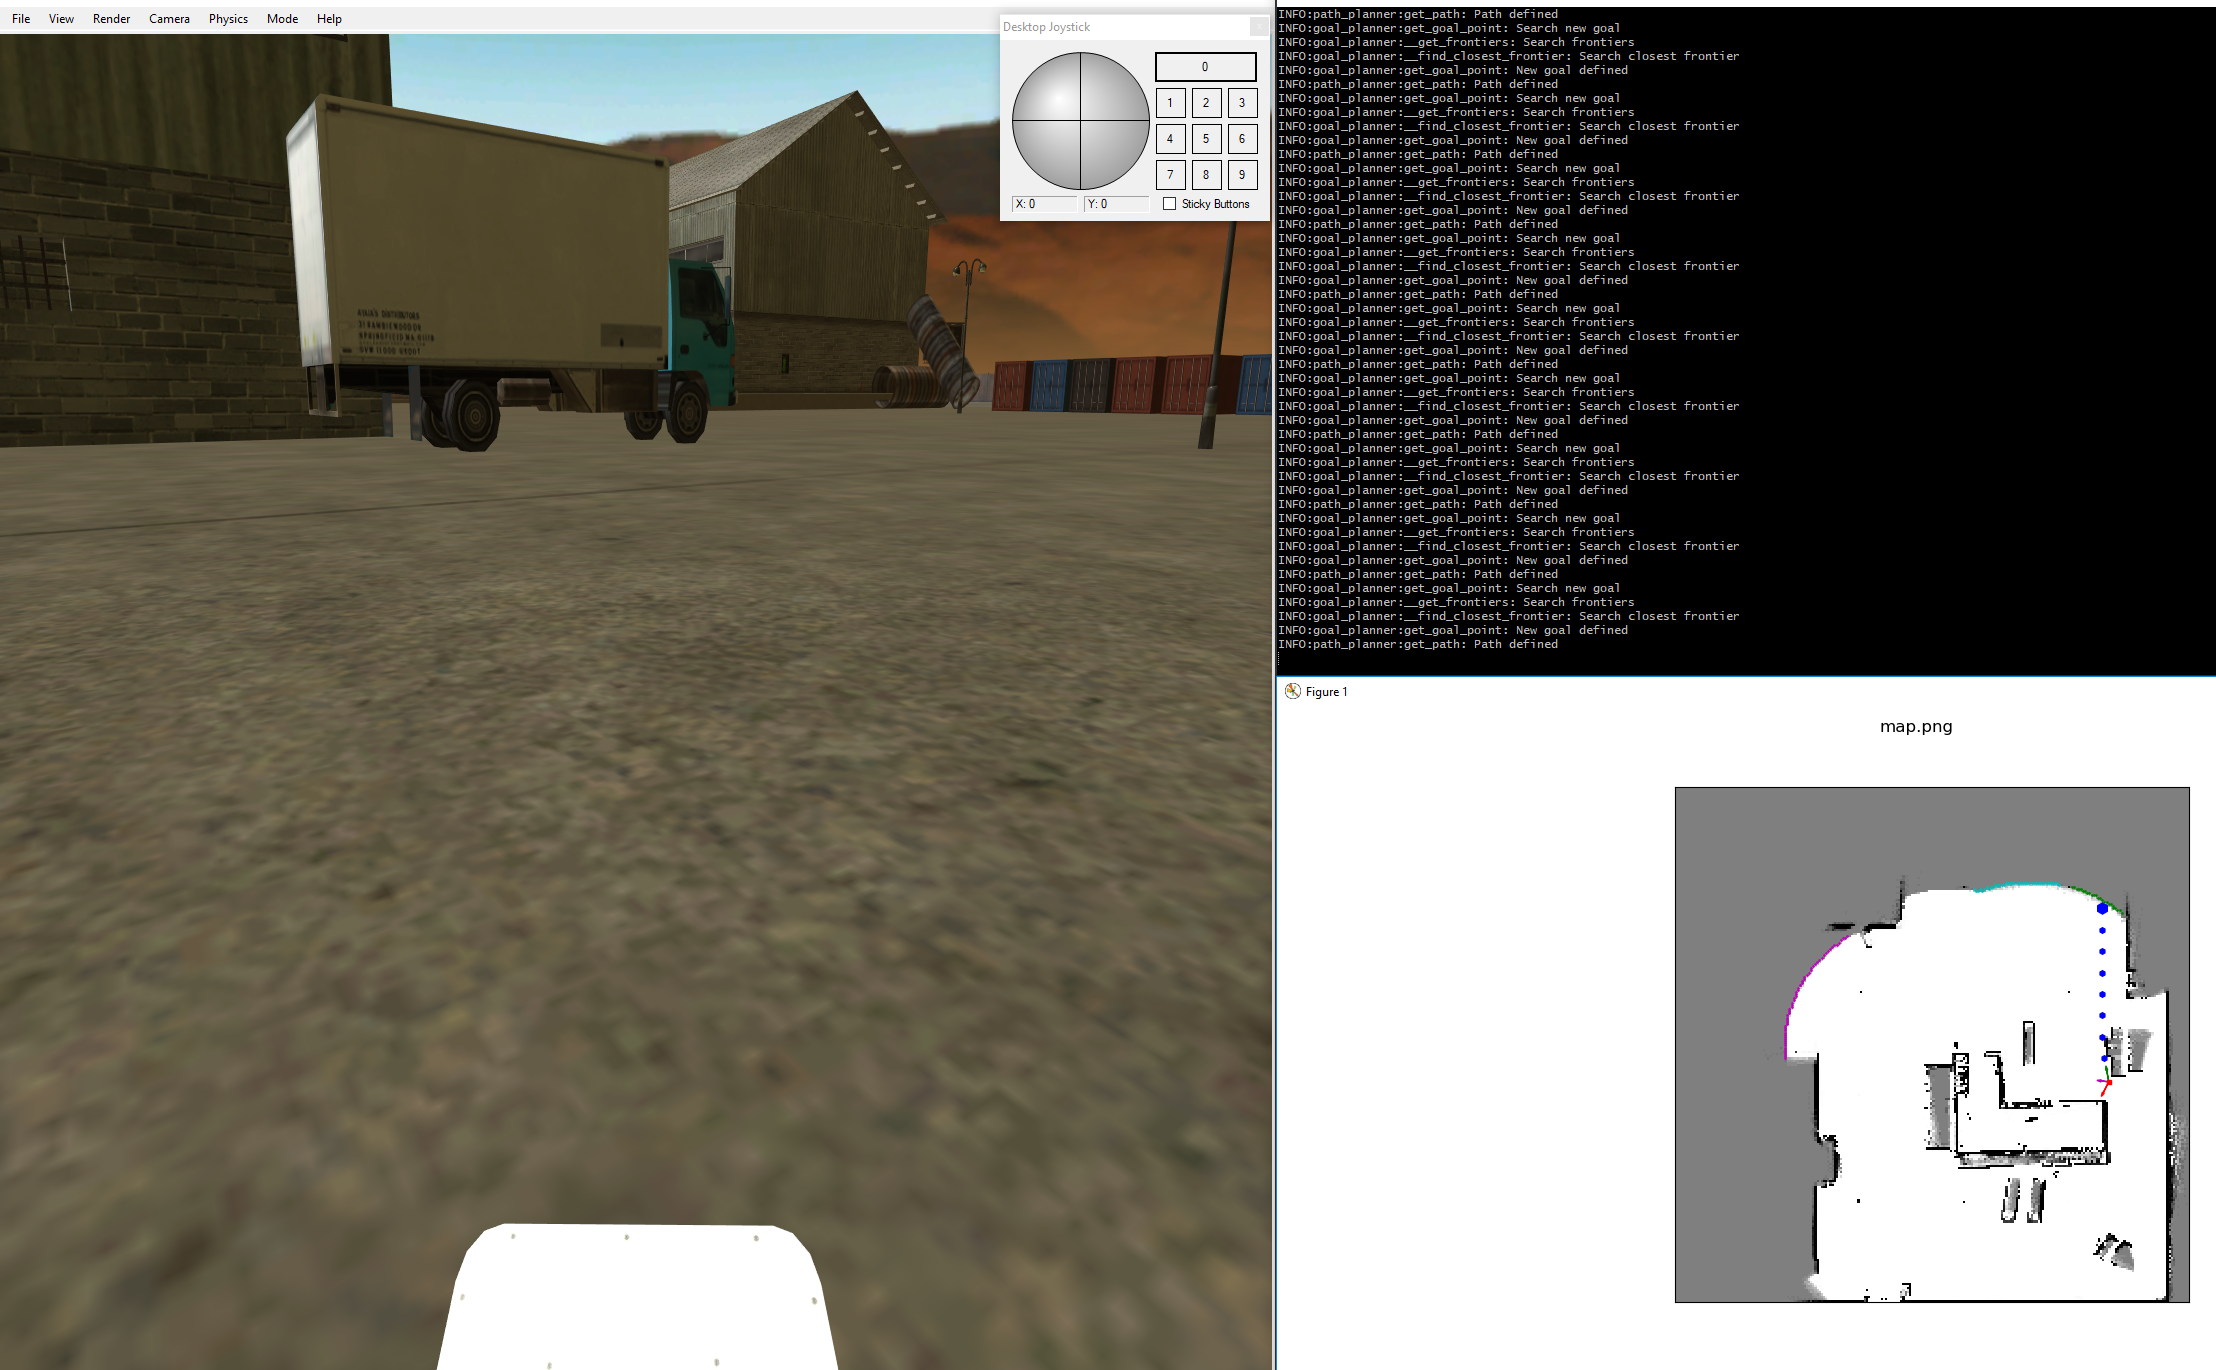
\includegraphics[width=\textwidth]{full_screen.png}
    \label{fig:full_screen}
    \caption{Full screen}
\end{figure}
\FloatBarrier
